% Created by tikzDevice version 0.10.1 on 2018-06-27 15:40:42
% !TEX encoding = UTF-8 Unicode
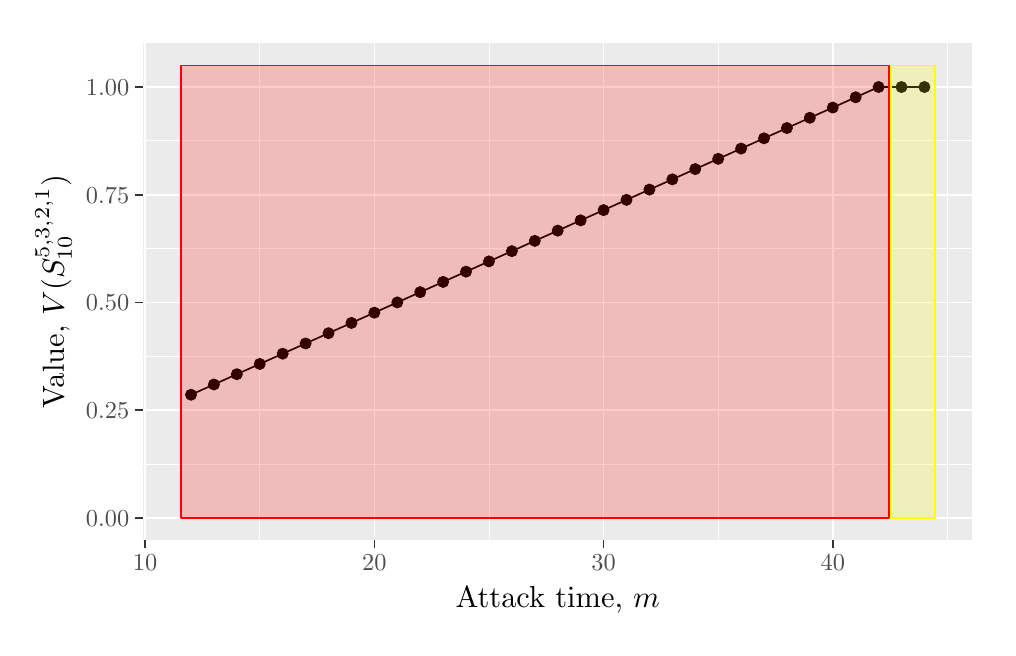
\begin{tikzpicture}[x=1pt,y=1pt]
\definecolor{fillColor}{RGB}{255,255,255}
\path[use as bounding box,fill=fillColor,fill opacity=0.00] (0,0) rectangle (346.90,216.81);
\begin{scope}
\path[clip] (  0.00,  0.00) rectangle (346.90,216.81);
\definecolor{drawColor}{RGB}{255,255,255}
\definecolor{fillColor}{RGB}{255,255,255}

\path[draw=drawColor,line width= 0.6pt,line join=round,line cap=round,fill=fillColor] (  0.00,  0.00) rectangle (346.90,216.81);
\end{scope}
\begin{scope}
\path[clip] ( 41.67, 31.53) rectangle (341.40,211.31);
\definecolor{fillColor}{gray}{0.92}

\path[fill=fillColor] ( 41.67, 31.53) rectangle (341.40,211.31);
\definecolor{drawColor}{RGB}{255,255,255}

\path[draw=drawColor,line width= 0.3pt,line join=round] ( 41.67, 59.16) --
	(341.40, 59.16);

\path[draw=drawColor,line width= 0.3pt,line join=round] ( 41.67, 98.07) --
	(341.40, 98.07);

\path[draw=drawColor,line width= 0.3pt,line join=round] ( 41.67,136.99) --
	(341.40,136.99);

\path[draw=drawColor,line width= 0.3pt,line join=round] ( 41.67,175.90) --
	(341.40,175.90);

\path[draw=drawColor,line width= 0.3pt,line join=round] ( 83.86, 31.53) --
	( 83.86,211.31);

\path[draw=drawColor,line width= 0.3pt,line join=round] (166.68, 31.53) --
	(166.68,211.31);

\path[draw=drawColor,line width= 0.3pt,line join=round] (249.51, 31.53) --
	(249.51,211.31);

\path[draw=drawColor,line width= 0.3pt,line join=round] (332.33, 31.53) --
	(332.33,211.31);

\path[draw=drawColor,line width= 0.6pt,line join=round] ( 41.67, 39.70) --
	(341.40, 39.70);

\path[draw=drawColor,line width= 0.6pt,line join=round] ( 41.67, 78.62) --
	(341.40, 78.62);

\path[draw=drawColor,line width= 0.6pt,line join=round] ( 41.67,117.53) --
	(341.40,117.53);

\path[draw=drawColor,line width= 0.6pt,line join=round] ( 41.67,156.44) --
	(341.40,156.44);

\path[draw=drawColor,line width= 0.6pt,line join=round] ( 41.67,195.36) --
	(341.40,195.36);

\path[draw=drawColor,line width= 0.6pt,line join=round] ( 42.45, 31.53) --
	( 42.45,211.31);

\path[draw=drawColor,line width= 0.6pt,line join=round] (125.27, 31.53) --
	(125.27,211.31);

\path[draw=drawColor,line width= 0.6pt,line join=round] (208.10, 31.53) --
	(208.10,211.31);

\path[draw=drawColor,line width= 0.6pt,line join=round] (290.92, 31.53) --
	(290.92,211.31);
\definecolor{drawColor}{RGB}{0,0,0}
\definecolor{fillColor}{RGB}{0,0,0}

\path[draw=drawColor,line width= 0.4pt,line join=round,line cap=round,fill=fillColor] (315.76,195.36) circle (  1.96);

\path[draw=drawColor,line width= 0.4pt,line join=round,line cap=round,fill=fillColor] (324.04,195.36) circle (  1.96);

\path[draw=drawColor,line width= 0.4pt,line join=round,line cap=round,fill=fillColor] ( 59.02, 84.17) circle (  1.96);

\path[draw=drawColor,line width= 0.4pt,line join=round,line cap=round,fill=fillColor] ( 67.30, 87.88) circle (  1.96);

\path[draw=drawColor,line width= 0.4pt,line join=round,line cap=round,fill=fillColor] ( 75.58, 91.59) circle (  1.96);

\path[draw=drawColor,line width= 0.4pt,line join=round,line cap=round,fill=fillColor] ( 83.86, 95.29) circle (  1.96);

\path[draw=drawColor,line width= 0.4pt,line join=round,line cap=round,fill=fillColor] ( 92.15, 99.00) circle (  1.96);

\path[draw=drawColor,line width= 0.4pt,line join=round,line cap=round,fill=fillColor] (100.43,102.70) circle (  1.96);

\path[draw=drawColor,line width= 0.4pt,line join=round,line cap=round,fill=fillColor] (108.71,106.41) circle (  1.96);

\path[draw=drawColor,line width= 0.4pt,line join=round,line cap=round,fill=fillColor] (116.99,110.12) circle (  1.96);

\path[draw=drawColor,line width= 0.4pt,line join=round,line cap=round,fill=fillColor] (125.27,113.82) circle (  1.96);

\path[draw=drawColor,line width= 0.4pt,line join=round,line cap=round,fill=fillColor] (133.56,117.53) circle (  1.96);

\path[draw=drawColor,line width= 0.4pt,line join=round,line cap=round,fill=fillColor] (141.84,121.24) circle (  1.96);

\path[draw=drawColor,line width= 0.4pt,line join=round,line cap=round,fill=fillColor] (150.12,124.94) circle (  1.96);

\path[draw=drawColor,line width= 0.4pt,line join=round,line cap=round,fill=fillColor] (158.40,128.65) circle (  1.96);

\path[draw=drawColor,line width= 0.4pt,line join=round,line cap=round,fill=fillColor] (166.68,132.35) circle (  1.96);

\path[draw=drawColor,line width= 0.4pt,line join=round,line cap=round,fill=fillColor] (174.97,136.06) circle (  1.96);

\path[draw=drawColor,line width= 0.4pt,line join=round,line cap=round,fill=fillColor] (183.25,139.77) circle (  1.96);

\path[draw=drawColor,line width= 0.4pt,line join=round,line cap=round,fill=fillColor] (191.53,143.47) circle (  1.96);

\path[draw=drawColor,line width= 0.4pt,line join=round,line cap=round,fill=fillColor] (199.81,147.18) circle (  1.96);

\path[draw=drawColor,line width= 0.4pt,line join=round,line cap=round,fill=fillColor] (208.10,150.88) circle (  1.96);

\path[draw=drawColor,line width= 0.4pt,line join=round,line cap=round,fill=fillColor] (216.38,154.59) circle (  1.96);

\path[draw=drawColor,line width= 0.4pt,line join=round,line cap=round,fill=fillColor] (224.66,158.30) circle (  1.96);

\path[draw=drawColor,line width= 0.4pt,line join=round,line cap=round,fill=fillColor] (232.94,162.00) circle (  1.96);

\path[draw=drawColor,line width= 0.4pt,line join=round,line cap=round,fill=fillColor] (241.22,165.71) circle (  1.96);

\path[draw=drawColor,line width= 0.4pt,line join=round,line cap=round,fill=fillColor] (249.51,169.41) circle (  1.96);

\path[draw=drawColor,line width= 0.4pt,line join=round,line cap=round,fill=fillColor] (257.79,173.12) circle (  1.96);

\path[draw=drawColor,line width= 0.4pt,line join=round,line cap=round,fill=fillColor] (266.07,176.83) circle (  1.96);

\path[draw=drawColor,line width= 0.4pt,line join=round,line cap=round,fill=fillColor] (274.35,180.53) circle (  1.96);

\path[draw=drawColor,line width= 0.4pt,line join=round,line cap=round,fill=fillColor] (282.63,184.24) circle (  1.96);

\path[draw=drawColor,line width= 0.4pt,line join=round,line cap=round,fill=fillColor] (290.92,187.94) circle (  1.96);

\path[draw=drawColor,line width= 0.4pt,line join=round,line cap=round,fill=fillColor] (299.20,191.65) circle (  1.96);

\path[draw=drawColor,line width= 0.4pt,line join=round,line cap=round,fill=fillColor] (307.48,195.36) circle (  1.96);

\path[draw=drawColor,line width= 0.6pt,line join=round] ( 59.02, 84.17) --
	( 67.30, 87.88) --
	( 75.58, 91.59) --
	( 83.86, 95.29) --
	( 92.15, 99.00) --
	(100.43,102.70) --
	(108.71,106.41) --
	(116.99,110.12) --
	(125.27,113.82) --
	(133.56,117.53) --
	(141.84,121.24) --
	(150.12,124.94) --
	(158.40,128.65) --
	(166.68,132.35) --
	(174.97,136.06) --
	(183.25,139.77) --
	(191.53,143.47) --
	(199.81,147.18) --
	(208.10,150.88) --
	(216.38,154.59) --
	(224.66,158.30) --
	(232.94,162.00) --
	(241.22,165.71) --
	(249.51,169.41) --
	(257.79,173.12) --
	(266.07,176.83) --
	(274.35,180.53) --
	(282.63,184.24) --
	(290.92,187.94) --
	(299.20,191.65) --
	(307.48,195.36) --
	(315.76,195.36) --
	(324.04,195.36);
\definecolor{drawColor}{RGB}{255,255,0}
\definecolor{fillColor}{RGB}{255,255,0}

\path[draw=drawColor,line width= 0.6pt,line join=round,fill=fillColor,fill opacity=0.20] (312.04, 39.70) rectangle (327.77,203.14);
\definecolor{drawColor}{RGB}{255,0,0}
\definecolor{fillColor}{RGB}{255,0,0}

\path[draw=drawColor,line width= 0.6pt,line join=round,fill=fillColor,fill opacity=0.20] ( 55.29, 39.70) rectangle (311.21,203.14);
\end{scope}
\begin{scope}
\path[clip] (  0.00,  0.00) rectangle (346.90,216.81);
\definecolor{drawColor}{gray}{0.30}

\node[text=drawColor,anchor=base east,inner sep=0pt, outer sep=0pt, scale=  0.88] at ( 36.72, 36.67) {0.00};

\node[text=drawColor,anchor=base east,inner sep=0pt, outer sep=0pt, scale=  0.88] at ( 36.72, 75.59) {0.25};

\node[text=drawColor,anchor=base east,inner sep=0pt, outer sep=0pt, scale=  0.88] at ( 36.72,114.50) {0.50};

\node[text=drawColor,anchor=base east,inner sep=0pt, outer sep=0pt, scale=  0.88] at ( 36.72,153.41) {0.75};

\node[text=drawColor,anchor=base east,inner sep=0pt, outer sep=0pt, scale=  0.88] at ( 36.72,192.33) {1.00};
\end{scope}
\begin{scope}
\path[clip] (  0.00,  0.00) rectangle (346.90,216.81);
\definecolor{drawColor}{gray}{0.20}

\path[draw=drawColor,line width= 0.6pt,line join=round] ( 38.92, 39.70) --
	( 41.67, 39.70);

\path[draw=drawColor,line width= 0.6pt,line join=round] ( 38.92, 78.62) --
	( 41.67, 78.62);

\path[draw=drawColor,line width= 0.6pt,line join=round] ( 38.92,117.53) --
	( 41.67,117.53);

\path[draw=drawColor,line width= 0.6pt,line join=round] ( 38.92,156.44) --
	( 41.67,156.44);

\path[draw=drawColor,line width= 0.6pt,line join=round] ( 38.92,195.36) --
	( 41.67,195.36);
\end{scope}
\begin{scope}
\path[clip] (  0.00,  0.00) rectangle (346.90,216.81);
\definecolor{drawColor}{gray}{0.20}

\path[draw=drawColor,line width= 0.6pt,line join=round] ( 42.45, 28.78) --
	( 42.45, 31.53);

\path[draw=drawColor,line width= 0.6pt,line join=round] (125.27, 28.78) --
	(125.27, 31.53);

\path[draw=drawColor,line width= 0.6pt,line join=round] (208.10, 28.78) --
	(208.10, 31.53);

\path[draw=drawColor,line width= 0.6pt,line join=round] (290.92, 28.78) --
	(290.92, 31.53);
\end{scope}
\begin{scope}
\path[clip] (  0.00,  0.00) rectangle (346.90,216.81);
\definecolor{drawColor}{gray}{0.30}

\node[text=drawColor,anchor=base,inner sep=0pt, outer sep=0pt, scale=  0.88] at ( 42.45, 20.52) {10};

\node[text=drawColor,anchor=base,inner sep=0pt, outer sep=0pt, scale=  0.88] at (125.27, 20.52) {20};

\node[text=drawColor,anchor=base,inner sep=0pt, outer sep=0pt, scale=  0.88] at (208.10, 20.52) {30};

\node[text=drawColor,anchor=base,inner sep=0pt, outer sep=0pt, scale=  0.88] at (290.92, 20.52) {40};
\end{scope}
\begin{scope}
\path[clip] (  0.00,  0.00) rectangle (346.90,216.81);
\definecolor{drawColor}{RGB}{0,0,0}

\node[text=drawColor,anchor=base,inner sep=0pt, outer sep=0pt, scale=  1.10] at (191.53,  7.44) {Attack time, $m$};
\end{scope}
\begin{scope}
\path[clip] (  0.00,  0.00) rectangle (346.90,216.81);
\definecolor{drawColor}{RGB}{0,0,0}

\node[text=drawColor,rotate= 90.00,anchor=base,inner sep=0pt, outer sep=0pt, scale=  1.10] at ( 13.08,121.42) {Value, $V(S_{ 10 }^{ 5, 3, 2, 1 })$};
\end{scope}
\end{tikzpicture}
